%%%%%%%%%%%%%%%%%%%%%%%%%%%%%%%%%%%%%%%%%%%%%%%%%%%%%%
% A Beamer template for University of Wollongong     %
% Based on THU beamer theme                          %
% Author: Qiuyu Lu                                   %
% Date: July 2024                                    %
% LPPL Licensed.                                     %
%%%%%%%%%%%%%%%%%%%%%%%%%%%%%%%%%%%%%%%%%%%%%%%%%%%%%%
% Customized for Sharif University of Technology     %
%%%%%%%%%%%%%%%%%%%%%%%%%%%%%%%%%%%%%%%%%%%%%%%%%%%%%%


\documentclass[serif, aspectratio=169]{beamer}
%\documentclass[serif]{beamer}  % for 4:3 ratio
\usepackage[T1]{fontenc} 
\usepackage{fourier} % see "http://faq.ktug.org/wiki/uploads/MathFonts.pdf" for other options
\usepackage{hyperref}
\usepackage{latexsym,amsmath,xcolor,multicol,booktabs,calligra}
\usepackage{graphicx,pstricks,listings,stackengine}
\usepackage{lipsum}
\usepackage{tikz}
\usetikzlibrary{shapes.geometric} % Add this to include ellipse shapes
\usepackage{amsmath}
\usepackage{pgfplots}  % For plots
\usepackage{amsmath}   % For equations
\usepackage{array}     % For tables
\pgfplotsset{compat=1.16}

% \usetikzlibrary{positioning}


\author{Ali Sharifi-Zarchi}
\title{Machine Learning (CE 40717)}
\subtitle{Fall 2024}
\institute{
    CE Department \\
    Sharif University of Technology
}
%\date{\small \today}
% \usepackage{UoWstyle}
\usepackage{SUTstyle}

% defs
\def\cmd#1{\texttt{\color{red}\footnotesize $\backslash$#1}}
\def\env#1{\texttt{\color{blue}\footnotesize #1}}
\definecolor{deepblue}{rgb}{0,0,0.5}
\definecolor{deepred}{RGB}{153,0,0}
\definecolor{deepgreen}{rgb}{0,0.5,0}
\definecolor{halfgray}{gray}{0.55}

\lstset{
    basicstyle=\ttfamily\small,
    keywordstyle=\bfseries\color{deepblue},
    emphstyle=\ttfamily\color{deepred},    % Custom highlighting style
    stringstyle=\color{deepgreen},
    numbers=left,
    numberstyle=\small\color{halfgray},
    rulesepcolor=\color{red!20!green!20!blue!20},
    frame=shadowbox,
}

\begin{document}

\begin{frame}
    \titlepage
    \vspace*{-0.6cm}
    \begin{figure}[htpb]
        \begin{center}
            
\includegraphics[keepaspectratio, scale=0.25]{pic/sharif-main-logo.png}
        \end{center}
    \end{figure}
\end{frame}

\begin{frame}    
\tableofcontents[sectionstyle=show,
subsectionstyle=show/shaded/hide,
subsubsectionstyle=show/shaded/hide]
\end{frame}

% ============================ Introduction ============================ 
\section{Introduction}

\begin{frame}{Self-Supervised Learning}
    \begin{picture}(0,0)
            \put(200,-150){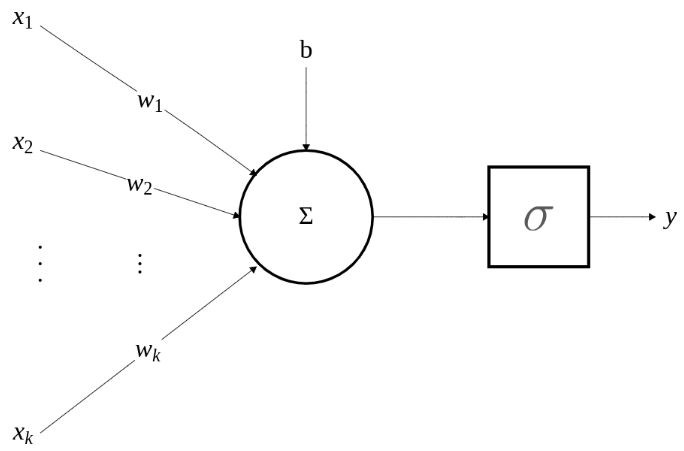
\includegraphics[width=7cm]{pic/1/neuron.png}} % Adjust path and size
    \end{picture}
     “the dark matter of intelligence” \footnote{\url{https://ai.meta.com/blog/self-supervised-learning-the-dark-matter-of-intelligence/}}
    \begin{itemize}
        \item $\{x_1, x_2, \dots, x_k\}$ : input features
        \item $\{w_1, w_2, \dots, w_k\}$ : feature weights
        \item $b$ : bias term
        \item $\sigma(\cdot)$ : activation function
        \item $y$ : output of the neuron
    \end{itemize}
\end{frame}

\begin{frame}{Self-Supervised Learning}
    \begin{center}
        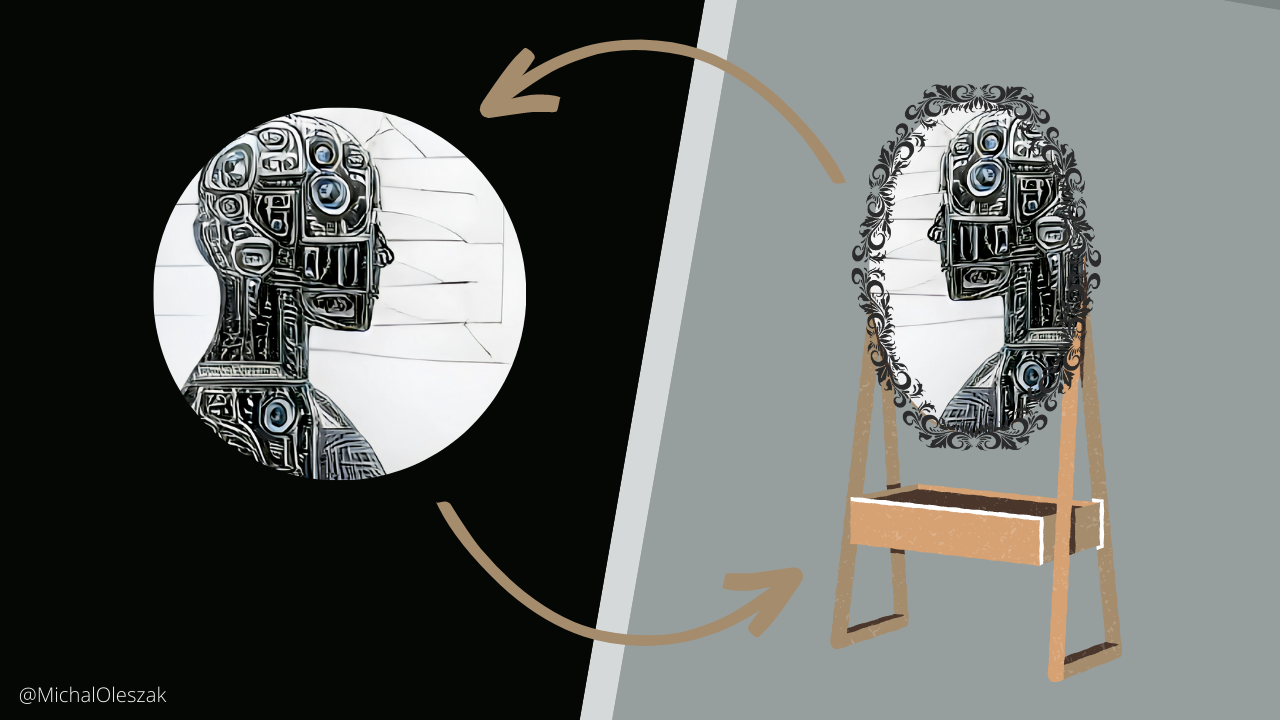
\includegraphics[width=0.6\textwidth]{pic/Intro.png} % Replace with the path to your image
        \\[1cm] % Adds space between image and quote
        \textit{“the dark matter of intelligence”}\footnote{\scriptsize \url{https://ai.meta.com/blog/self-supervised-learning-the-dark-matter-of-intelligence/}}
    \end{center}
\end{frame}

\begin{frame}{Why Neural Networks?}
    \begin{itemize}
        \item  Self-supervised learning defines a \textbf{pretext} task based on unlabeled inputs to produce descriptive and intelligible representations [Hastie et al., 2009, Goodfellow et al., 2016]
        \begin{itemize}
            \item Learn with supervised learning objectives, e.g., classification, regression.
	\item Labels of these pretext tasks are generated \textit{automatically}
	\item Can be used in other downstream tasks.
        \end{itemize}
    \end{itemize}
\end{frame}


\begin{frame}[t]{Example Workflow}
    
    \begin{itemize}
\item Training objective: predicting the context surrounding a word
\item encourages the model to capture relationships among words
\item The same SSL model representations can be used across a range
 of downstream tasks. e.g.
        \begin{itemize}
	\item translating text across languages
	\item summarizing
	\item generating text
        \end{itemize}
    \end{itemize}

\end{frame}

\begin{frame}[t]{Motivation}
  
    \begin{itemize}
        \item Problem: Supervised Learning is Expensive!
            \begin{itemize}
        \item Labeling data is costly
\item SSL: Use signals that can be created automatically from data.
    \end{itemize}
\item Labled data is harder to find. There is much more unlabled data.
\item Supervised Learning is not how \textbf{we} learn
  \begin{itemize}
 \item Babies don’t get supervision for everything they see!

     \end{itemize}

    \end{itemize}

\end{frame}



\begin{frame}[t]{Comparison}
Methods that learn from data without annotations.
    \begin{itemize}
        
\item \textbf{ Unsupervised Learning}: Model isn’t told what to predict. Older 
terminology, not used as much today.
 \item \textbf{ Self-Supervised Learning}: Model is trained to predict some naturally
occurring signal in the raw data rather than human annotations.
 \item \textbf{  Semi-Supervised Learning}: Train jointly with some labeled data and (a lot)
 of unlabeled data
    \end{itemize}
\end{frame}

\iffalse
\begin{frame}{Comparison of Learning Paradigms}

    \begin{center}
        \begin{tabular}{|c|c|c|c|}
            \hline
            \textbf{Aspect} & \textbf{Supervised} & \textbf{Unsupervised} & \textbf{Self-Supervised} \\ \hline
            \textbf{Data Labels} & Required & Not Required & Pseudo-Labels \\ \hline
            \textbf{Goal} & Predict labels & Find patterns/structure & Learn representations \\ \hline
            \textbf{Example Tasks} & Classification, Regression & Clustering, Dimensionality Reduction & Pretraining for downstream tasks \\ \hline
            \textbf{Examples} & Image classification, spam detection & K-means, PCA & BERT, SimCLR \\ \hline
            \textbf{Strengths} & Accurate when data is labeled & Useful when labels are scarce & Leverages unlabeled data effectively \\ \hline
            \textbf{Weaknesses} & Requires labeled data & Limited to pattern discovery & Requires complex pseudo-label generation \\ \hline
        \end{tabular}
    \end{center}
\end{frame}
\fi

\iffalse
\begin{frame}{Comparison of Learning Paradigms}
(COMMENTED SLIDE)
    \begin{center}
        \begin{tabular}{l l l l}
            \textbf{Aspect} & \textbf{Supervised} & \textbf{Unsupervised} & \textbf{Self-Supervised} \\[0.3cm]
            \hline \\[-0.3cm]
            \textbf{Data Labels} & Required & Not Required & Pseudo-Labels \\[0.3cm]
            \textbf{Goal} & Predict labels & Find patterns/structure & Learn representations \\[0.3cm]
            \textbf{Example Tasks} & Classification, Regression & Clustering, Dimensionality Reduction & Pretraining for downstream tasks \\[0.3cm]
            \textbf{Examples} & Image classification, spam detection & K-means, PCA & BERT, SimCLR \\[0.3cm]
            \textbf{Strengths} & Accurate when data is labeled & Useful when labels are scarce & Leverages unlabeled data effectively \\[0.3cm]
            \textbf{Weaknesses} & Requires labeled data & Limited to pattern discovery & Requires complex pseudo-label generation \\[0.3cm]
        \end{tabular}
    \end{center}
\end{frame}
\fi

%


\begin{frame}{Evaluation}
    \begin{itemize}
       \item We usually don’t care about the performance of the self-supervised learning task, e.g., we don’t care if the model learns to predict image 
rotation perfectly.
 \item Evaluate the learned feature encoders on downstream target tasks

    \end{itemize}
\end{frame}

\begin{frame}{Evaluation Cont.}
        
     \begin{flushleft}
           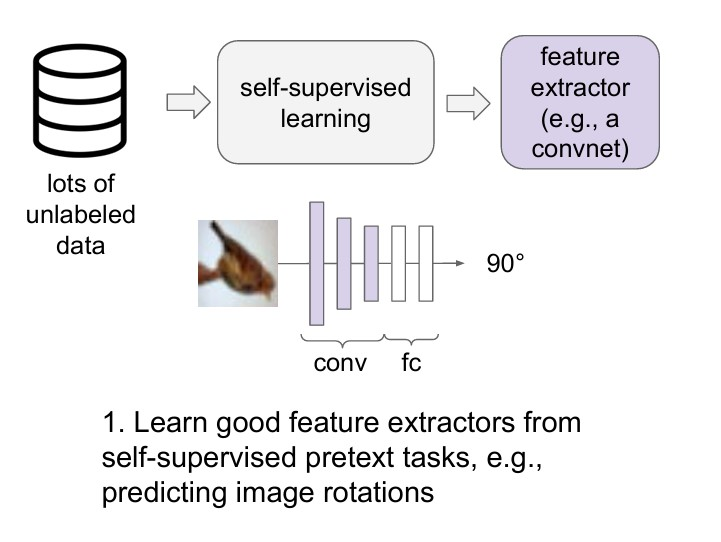
\includegraphics[keepaspectratio, scale=0.5]{pic/Evaluation-1.jpg}
\end{flushleft}
  
\end{frame}


\begin{frame}{Evaluation Cont.}
        \begin{figure}[htpb]
   
           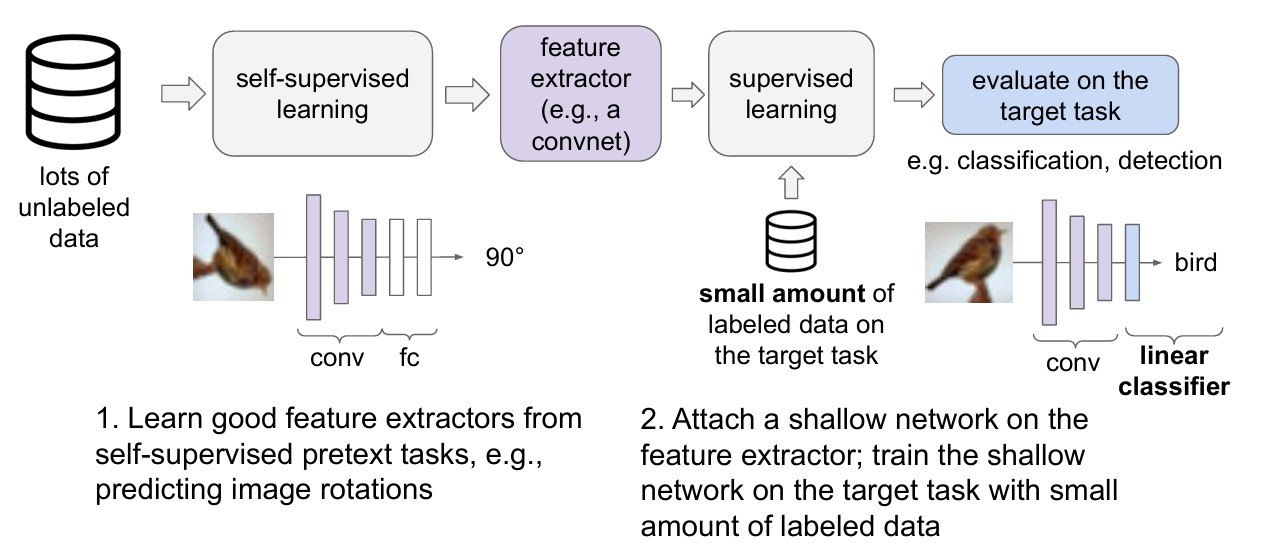
\includegraphics[keepaspectratio, scale=0.5]{pic/Evaluation-2.jpg}

    \end{figure}
\end{frame}


\begin{frame}{Example}
      \begin{itemize}
 \item Pretext task: predict rotations
\item  Hypothesis: a model could recognize the correct rotation of an object 
only if it has the “visual commonsense” of what the object should look 
like unperturbed.
\item The model learns to 
predict which rotation 
is applied (4-way 
classification)
\item (This slide will be ellaborated on and expanded with diagrams)

  \end{itemize}
\end{frame}

\section{Multimodality}


\begin{frame}{Idea}
     
 \begin{itemize}
 % \item    Many papers would pretrain on (unlabeled) ImageNet, then evaluate on ImageNet!
 %     \begin{itemize}
 %         \item Potential bias
 %         \item Does not truly test the generalizability of the learned representations
 %     \end{itemize}
 \item  Don’t learn from isolated images -- take images together with some \textbf{context}
\item \textbf{Video}: Image together with adjacent video frames
 \item \textbf{Sound}: Image with audio track from video
 \item \textbf{3D Image}: Image with depth map or point cloud
\item  \color{purple}{\textbf{Language:} Image with natural-language text (e.g., captions or descriptions)}

  \end{itemize}
\end{frame}

\begin{frame}{Why Language?}
        \begin{itemize}
          \item \textbf{Rich Semantics}
          \begin{itemize}
              \item Just a few words give rich information.
              \item Acts as a bridge between sensory data and abstract human understanding.
          \end{itemize}
          
          \item  \textbf{Universality}
          \begin{itemize}
              \item Language can describe almost any concept
              \item Language can act as a \textbf{universal medium} for aligning other modalities, even structured data.
          \end{itemize} 
        \end{itemize}
\end{frame}


\begin{frame}{Why Language? (Cont.)}
        \begin{itemize}
          \item \textbf{Large-Scale Data Availability}
          \begin{itemize}
              \item The internet contains vast amounts of textual data.
              \item Text data is relatively easier to collect, clean, and annotate (no need to experts) compared to modalities like video or audio.
              \item Available datasets such as COCO (images and captions)
          \end{itemize}

          \item \textbf{Pretrained Language Models (PLMs) as a Strong Foundation}
          \begin{itemize}
              \item Large pretrained language models with remarkable capabilities.
              \item Language models are highly transferable (transfer learning) across tasks, enabling multimodal systems to adapt to various downstream applications efficiently.
          \end{itemize}
        \end{itemize}
\end{frame}


\section{Contrastive Learning}


\begin{frame}{Definition}
    \begin{itemize}
        \item A machine learning technique for training models to distinguish between similar and dissimilar data points.

        \item \textbf{Key Idea}
        \begin{itemize}
            \item Bring similar data points closer in the embedding space.
            \item Push dissimilar data points farther apart.
        \end{itemize}
    \end{itemize}
\end{frame}


\begin{frame}{Definition (Cont.)}
    \begin{itemize}
        \item \textbf{Purpose:} Learn meaningful representations for downstream tasks like classification, clustering, or retrieval
        \item \textbf{Widely Used In:} Representation learning across domains such as computer vision, NLP, and multi-modal tasks.
    \end{itemize}
\end{frame}


\begin{frame}{Key Concepts}
    \begin{itemize}
        \item \textbf{Embedding Space}
        \begin{itemize}
            \item The data points are mapped into a high-dimensional space, called the embedding space.
            \item Their relative positions encode similarity or dissimilarity.
        \end{itemize}
        
        \item \textbf{Positive Pairs:} Data points that are semantically similar.
        \item \textbf{Negative Pairs:} Data points that are semantically different.
    \end{itemize}
\end{frame}


\begin{frame}{Key Concepts (Cont.)}
    \begin{itemize}
        \item \textbf{Objectives}
        \begin{itemize}
            \item Minimize the distance between the embeddings of positive pairs.
            \item Maximize the distance between the embeddings of negative pairs.
        \end{itemize}

        \item \textbf{Loss Functions:} We'll discuss 2 most commonly used loss functions in contrastive learning in the following slides.
    \end{itemize}
\end{frame}


\begin{frame}{Loss Functions - Contrastive Loss
 \footnote{\href{http://yann.lecun.com/exdb/publis/pdf/hadsell-chopra-lecun-06.pdf}{Dimensionality Reduction by Learning an Invariant Mapping}}
 \footnote{\href{https://medium.com/@maksym.bekuzarov/losses-explained-contrastive-loss-f8f57fe32246}{Losses explained: Contrastive Loss}}
}
     \begin{itemize}
         \item Contrastive loss was first introduced in 2005 by Yann Le Cunn et al.
         \item Its original application was in Dimensionality Reduction.
     \end{itemize}
\end{frame}


\begin{frame}{Loss Functions - Contrastive Loss (Cont.)}
\begin{equation*}
D_W\left(\vec{X}_1, \vec{X}_2\right)=\left\|G_W\left(\vec{X}_1\right)-G_W\left(\vec{X}_2\right)\right\|_2
\end{equation*}

    \begin{itemize}
        \item $D_W\left(\vec{X}_1, \vec{X}_2\right)$ is dissimilarity between the two data points $\vec{X}_1$ and $\vec{X}_2$.
        \item $G_W$ is a transformation function (e.g., a neural network) parameterized by $W$.
        \item Generally, $D_W$ can be any metric that indicates the dissimilarity between $\vec{X}_1$ and $\vec{X}_2$.
    \end{itemize}
\end{frame}


\begin{frame}{Loss Functions - Contrastive Loss (Cont.)}
\begin{equation*}
L\left(W,\left(Y, \vec{X}_1, \vec{X}_2\right)^i\right)=(1-Y) L_S\left(D_W^i\right)+Y L_D\left(D_W^i\right)
\end{equation*}

    \begin{itemize}
        \item $\left(Y, \vec{X}_1, \vec{X}_2\right)^i$ is the $i$-th labeled sample pair.
        \item $Y=0$ if $\vec{X}_1$ and $\vec{X}_2$ are deemed similar, and $Y=1$ if they are deemed dissimilar.
        \item $L_S$ is the partial loss function for a pair of similar points.
        \item $L_D$ is the partial loss function for a pair of dissimilar points.
        \item $L_S$ and $L_D$ must be properly designed to reduce $L$.
    \end{itemize}
\end{frame}


\begin{frame}{Loss Functions - Contrastive Loss (Cont.)}
\begin{equation*}
\mathcal{L}(W)=\sum_{i=1}^P L\left(W,\left(Y, \vec{X}_1, \vec{X}_2\right)^i\right)
\end{equation*}

    \begin{itemize}
        \item $P$ is the number of training pairs (which may be as large as the
square of the number of samples).
    \end{itemize}
\end{frame}


 \begin{frame}{Loss Functions - InfoNCE Loss\footnote{\href{https://arxiv.org/pdf/1807.03748v2}{Representation Learning with Contrastive Predictive Coding}}}
     \begin{itemize}
         \item First, we'll explore this loss from a theoretical perspective which has been discussed in its original paper.
         \item Next, we'll discuss how it can be applied in practice.
     \end{itemize}
 \end{frame}


\begin{frame}{Loss Functions - InfoNCE Loss (Cont.)}
     \begin{itemize}
         \item It's the loss in its original paper:
     \end{itemize}

     \begin{equation*}
         \mathcal{L}_{\mathrm{N}}=-{\mathbb{E}_X}\left[\log \frac
         {\frac{p\left(x_{t+k} \mid c_t\right)}{p\left(x_{t+k}\right)}}
         {\sum_{x_j \in X} \frac{p\left(x_{t} \mid c_t\right)}{p\left(x_{t}\right)}}
         \right]
     \end{equation*}
\end{frame}


\begin{frame}{Loss Functions - InfoNCE Loss (Cont.)}
     \begin{itemize}
         \item Let's start with mutual information.
         \item We have a set $X=\left\{x_1, \ldots, x_N\right\}$ of $N$ random samples containing one positive sample from $p\left(x_{t+k} \mid c_t\right)$ and $N - 1$ negative samples from the \textbf{proposal} distribution $p\left(x_{t+k}\right)$
         \item Our purpose is to maximize mutual information:
     \end{itemize}

     \begin{equation*}
         I(x_{t+k}; c_t)=\sum_{x_{t+k}, c_t} p(x_{t+k}, c_t) \log \frac{p(x_{t+k} \mid c_t)}{p(x_{t+k})}
     \end{equation*}

     \begin{itemize}
         \item $c_t$ is context latent representation.
     \end{itemize}
\end{frame}


\begin{frame}{Loss Functions - InfoNCE Loss (Cont.)}
     \begin{itemize}
         \item We know:
     \end{itemize}

     \begin{equation*}
         I(x_{t+k}; c_t) \leq \log N \xrightarrow{} I(x_{t+k}; c_t) \geq \log N - \mathcal{L}_{\mathrm{N}}
     \end{equation*}

     \begin{itemize}
         \item $\mathcal{L}_{\mathrm{N}}$ quantifies the gap between the true mutual information and the approximation.
         \item Minimizing $\mathcal{L}_{\mathrm{N}}$ effectively maximizes the mutual information.
     \end{itemize}
\end{frame}


\begin{frame}{Loss Functions - InfoNCE Loss (Cont.)}
     \begin{itemize}
         \item Categorical cross-entropy of classifying the positive sample correctly, with $\frac{f_k}{\sum_X f_k}$ being the prediction of the model.
     \end{itemize}

     \begin{equation*}
         \mathcal{L}_{\mathrm{N}}=-{\mathbb{E}_X}\left[\log \frac{f_k\left(x_{t+k}, c_t\right)}{\sum_{x_j \in X} f_k\left(x_j, c_t\right)}\right]
     \end{equation*}

     \begin{itemize}
         \item We want to optimize it.
     \end{itemize}
\end{frame}


\begin{frame}{Loss Functions - InfoNCE Loss (Cont.)}
     \begin{itemize}
         \item Let's write the optimal probability for this loss as $p\left(d=i \mid X, c_t\right)$ with $[d=i]$ being the indicator that sample $x_i$ is the \textbf{positive} sample.
         \item The probability that sample $x_i$ was drawn from the conditional distribution $p\left(x_{t+k} \mid c_t\right)$ rather than the proposal distribution $p\left(x_{t+k}\right)$ can be derived as follows:
     \end{itemize}

     \begin{equation*}
         p\left(d=i \mid X, c_t\right)=
         \frac{p\left(x_i \mid c_t\right) \prod_{l \neq i} p\left(x_l\right)}{\sum_{j=1}^N p\left(x_j \mid c_t\right) \prod_{l \neq j} p\left(x_l\right)}=
         \frac{\frac{p\left(x_i \mid c_t\right)}{p\left(x_i\right)}}{\sum_{j=1}^N \frac{p\left(x_j \mid c_t\right)}{p\left(x_j\right)}}
     \end{equation*}

     \begin{itemize}
         \item As we can see, the optimal value for $f_k\left(x_{t+k}, c_t\right)$ in $\mathcal{L}_{\mathrm{N}}$ is proportional to $\frac{p\left(x_{t+k} \mid c_t\right)}{p\left(x_{t+k}\right)}$ and this is independent of the choice of the number of negative samples $N - 1$.
     \end{itemize}
\end{frame}


\begin{frame}{Loss Functions - InfoNCE Loss (Cont.)}
     \begin{itemize}
         \item We can evaluate the mutual information between the variables $c_t$ and $x_{t+k}$ as follows:
     \end{itemize}

     \begin{equation*}
         I\left(x_{t+k}, c_t\right) \geq \log (N)-\mathcal{L}_{\mathrm{N}}
     \end{equation*}

     \begin{itemize}
         \item It becomes tighter as $N$ becomes larger.
         \item Minimizing the InfoNCE loss $\mathcal{L}_{\mathrm{N}}$ maximizes a lower bound on mutual information.
     \end{itemize}
\end{frame}


\begin{frame}{Loss Functions - InfoNCE Loss (Cont.)}
     \begin{itemize}
         \item In practice, we have:
     \end{itemize}

     \begin{equation*}
         \mathcal{L}_{\mathrm{N}}=-\frac{1}{N} \sum_{i=1}^N \log \frac{\exp \left(\operatorname{sim}\left(x_i, c_i\right) / \tau\right)}{\sum_{j=1}^N \exp \left(\operatorname{sim}\left(x_i, c_j\right) / \tau\right)}
     \end{equation*}

     \begin{itemize}
         \item Used in models like SimCLR, MoCo, CLIP, and others.
         \item Next, we want to derive this formula from the theoretical one.
     \end{itemize}
\end{frame}


\begin{frame}{Loss Functions - InfoNCE Loss (Cont.)}
    \begin{itemize}
         \item \textbf{Step 1:}
     \end{itemize}

     \begin{equation*}
         \frac{p\left(x \mid c\right)}{p\left(x\right)} =
         \exp\left(\log \left(\frac{p\left(x \mid c\right)}{p\left(x\right)}\right) \right)
     \end{equation*}

     \begin{itemize}
         \item But in practice, we rarely know the true densities $p\left(x \mid c\right)$ and $p\left(x\right)$.
         \item Instead, we learn a function that approximates their log‐ratio.
         \item A common approach is to let a neural network produce embeddings $f\left(x\right)$ and $g\left(c\right)$.
     \end{itemize}
\end{frame}


\begin{frame}{Loss Functions - InfoNCE Loss (Cont.)}
    \begin{equation}
    \begin{split}
        \log \left(\frac{p\left(x \mid c\right)}{p\left(x\right)}\right) &\approx
        \operatorname{sim}\left(f\left(x\right), g\left(c\right) \right)    \xrightarrow{\text{we annotate it as}}
        \operatorname{sim}\left(x, c \right) \xrightarrow{} \\&
        \frac{p\left(x \mid c\right)}{p\left(x\right)} \approx
        \exp\left( \operatorname{sim}\left(x, c \right) \right)
    \end{split}
    \end{equation}

     \begin{itemize}
         \item $\operatorname{sim}\left(x, c \right)$ is similarity function (e.g., cosine similarity or dot product).
         \item Replacing unknown densities with a similarity function, yielding a \textbf{softmax} function (which we'll discuss).
         \item It’s straightforward to implement using standard deep‐learning toolkits.
     \end{itemize}
\end{frame}


\begin{frame}{Loss Functions - InfoNCE Loss (Cont.)}
    \begin{itemize}
        \item Why $\operatorname{sim}\left(x, c \right)$ works?

        \begin{itemize}
            \item It becomes large (positive) for the true \textbf{positive} pair $\left(x,c\right)$.
            \item It becomes relatively small (negative) for \textbf{negative} pairs $\left(x,c'\right)$.
        \end{itemize}

        \begin{equation*}
            \operatorname{sim}\left(x, c \right) \gg \operatorname{sim}\left(x, c' \right) \longleftrightarrow
            p\left(x, c \right) \gg p\left(x, c' \right)
        \end{equation*}

        \begin{itemize}
            \item This is the property required to approximate the ratio $p\left(x \mid c\right)/p\left(x\right)$.
        \end{itemize}
    \end{itemize}
\end{frame}


\begin{frame}{Loss Functions - InfoNCE Loss (Cont.)}
    \begin{itemize}
        \item \textbf{Step 2:}
        \item In practice, we don’t have the full distribution $X$ or its expectations.
        \item Instead, we approximate this using batches of size $N$.
        \item Each $x_{t+k}$ is treated as the \textbf{positive sample}, and the other $x_j$s in the batch are treated as \textbf{negative samples}.
        \item The expectation becomes a summation over batches:
    \end{itemize}

    \begin{equation}
        \mathcal{L}_{\mathrm{N}} =
        -{\mathbb{E}_X}\left[\log \frac{f_k\left(x_{t+k}, c_t\right)}{\sum_{x_j \in X} f_k\left(x_j, c_t\right)}\right] \approx
        -\frac{1}{N} \sum_{i=1}^N\log \frac{f_k\left(x_{t+k}, c_t\right)}{\sum_{x_j \in X} f_k\left(x_j, c_t\right)}
    \end{equation}
\end{frame}


\begin{frame}{Loss Functions - InfoNCE Loss (Cont.)}
    \begin{itemize}
        \item \textbf{Step 3:}
        \item To control the sharpness of the similarity distribution, a temperature parameter $\tau$ is introduced:
    \end{itemize}

    \begin{equation}
        \operatorname{sim}\left(x, c \right) \xrightarrow{}
        \frac{\operatorname{sim}\left(x, c \right)}{\tau}
    \end{equation}

    \begin{itemize}
        \item $\tau$ helps balance gradients during training:

        \begin{itemize}
            \item With no $\tau$, large similarity scores might dominate the gradients, leading to unstable updates.
            \item A carefully chosen $\tau$ scales the scores appropriately, ensuring stable convergence.
        \end{itemize}
    \end{itemize}
\end{frame}


\begin{frame}{Loss Functions - InfoNCE Loss (Cont.)}
    \begin{itemize}
        \item $\tau$ affects the distribution of similarity scores after applying the softmax function; in other words, it influences the sharpness of the softmax.
        
        \item Low $\tau$:
        \begin{itemize}
            \item High sharpness.
            \item The softmax heavily favors the largest score.
            \item The distribution becomes more concentrated on the top-scoring pair.
            \item Encourages the model to focus strongly on the positive sample while ignoring negatives.
            \item The loss becomes more sensitive to small differences in scores.
        \end{itemize}

        \item High $\tau$:
        \begin{itemize}
            \item Low sharpness.
            \item The softmax smooths the distribution, making it more uniform.
            \item This encourages the model to consider a broader set of samples, not just the top-scoring pair.
            \item Useful when the data is noisy or when the model needs to generalize better.
        \end{itemize}
    \end{itemize}
\end{frame}


\begin{frame}{Loss Functions - InfoNCE Loss (Cont.)}
    \begin{itemize}
        \item \textbf{Finally:} From equations (1) to (3), we derive:
    \end{itemize}

    \begin{equation*}
        \mathcal{L}_{\mathrm{N}}=-{\mathbb{E}_X}\left[\log \frac{f_k\left(x_{t+k}, c_t\right)}{\sum_{x_j \in X} f_k\left(x_j, c_t\right)}\right] \approx
        -\frac{1}{N} \sum_{i=1}^N \log \frac{\exp \left(\operatorname{sim}\left(x_i, c_i\right) / \tau\right)}{\sum_{j=1}^N \exp \left(\operatorname{sim}\left(x_i, c_j\right) / \tau\right)}
    \end{equation*}
\end{frame}



\begin{frame}{Common Components}
    \begin{itemize}
        \item Dataset :
\begin{itemize}
\item supervised:  $D_m = \{ (x_1^1, \cdots, x_M^1, y^1), \cdots, (x_1^n, \cdots, x_M^n, y^n)  \}$
\item self-supervised:  $D_m = \{ (x_1^1, \cdots, x_M^1), \cdots, (x_1^n, \cdots, x_M^n)  \}$
\end{itemize}
\item The psudo-label or signal generated for SSL can be denoted as $z = P(x_1,\cdot,x_M)$.

        \item Modality Encoder(s): $c = e_k(x_k^i; \theta_k)$ for each modality $k$.
	\item Fusion Module: $f_\psi$ to integrate the encoded information of different modalities
	\item Pretext task head (like a predictive head) : $g_\gamma$ and some SSL loss $\mathcal{L}_{SSL}$

    \end{itemize}
\end{frame}


\begin{frame}{Architectures}
  \begin{itemize}
\item There many veriations and structures
  \end{itemize}
 \begin{minipage}{0.48\textwidth} % Adjust the width as needed
        \begin{figure}
	\centering
        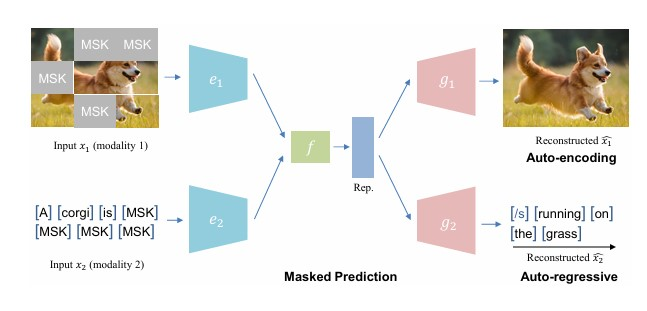
\includegraphics[width=\textwidth]{pic/SSL-MM-var1.jpg} % Replace with your image path
        \caption{Figure 1 masked prediction frameworks} % Optional
   \end{figure}
    \end{minipage} \hfill % Add some space between the two images
    \begin{minipage}{0.48\textwidth}
   \begin{figure}
        \centering
        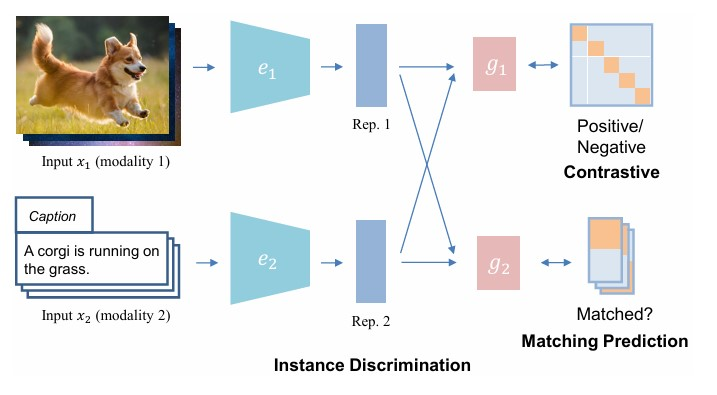
\includegraphics[width=\textwidth]{pic/SSL-MM-var2.jpg} % Replace with your image path
        \caption{Figure 2 instance discrimination objectives} % Optional
   \end{figure}
    \end{minipage}
\end{frame}


\begin{frame}{CLIP}
\begin{itemize}
\item Connecting text and images
\item Contrastive Language–Image Pre-training
\item CLIP $\implies$ a shared representation(embedding) between two modalities (text and images) by training on a large dataset of image-text pairs.
\end{itemize}
\end{frame}

\begin{frame}{CLIP Cont.}
\begin{itemize}
\item Image Encoder: a Vision Transformer (ViT) or a ResNet.
\item Text Encoder: A Transformer model 
\end{itemize}
\begin{figure}[hb]
        \begin{center}
            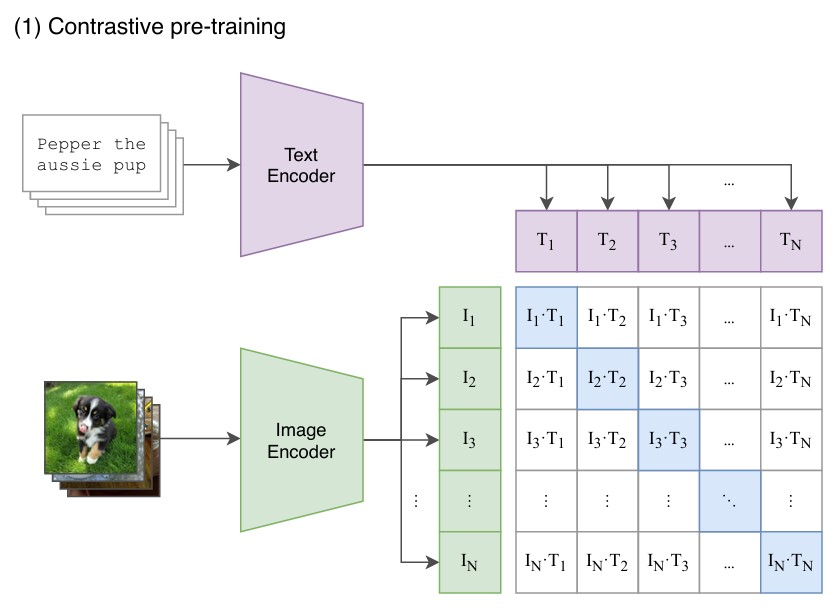
\includegraphics[keepaspectratio, scale=0.5]{pic/clip-overview.jpg}
        \end{center}
    \end{figure}
\end{frame}


\begin{frame}{CLIP Goals}
\begin{itemize}
\item CLIP was designed to mitigate a number of major problems:
\item Costly datasets: Deep learning needs a lot of data, manually labeled datasets are expensive to construct.
\begin{itemize}
\item CLIP learns from text–image pairs that are already publicly available on the internet
\end{itemize}
\item Narrow: An ImageNet model excels at predicting the 1000 ImageNet categories but requires additional data and fine-tuning for other tasks. 

\begin{itemize}
\item CLIP can be adapted to perform a wide variety of visual classification tasks without needing additional training examples. 
\end{itemize}
\end{itemize}

\end{frame}


\begin{frame}{Zero-Shot Classification}
\begin{itemize}
\item (Put Zero-Shot and Applications Slides here)
\end{itemize}
\end{frame}

\section{References}

\begin{frame}{Contributions}
\textbf{These slides are authored by:}
    \begin{itemize}
        \item Amir Mohammad Fakhimi
        \item Hooman Zolfaghari
    \end{itemize}
    
\end{frame}


\begin{frame}[allowframebreaks]
   \bibliographystyle{ieeetr} % Place the style before bibliography
   \bibliography{ref.bib} % Point to your .bib file
   \nocite{*} % Include all references even if not cited
\end{frame}


\end{document}


\begin{tikzpicture}[remember picture,overlay]
        \node[anchor=south west, xshift=0.3cm, yshift=0.3cm] at (current page.south west) {\tiny \href{https://medium.com/@maksym.bekuzarov/losses-explained-contrastive-loss-f8f57fe32246}{Medium: Losses explained: Contrastive Loss}};
    \end{tikzpicture}